\documentclass[10pt,t]{beamer}
\usepackage[utf8]{inputenc}
\usepackage[T1]{fontenc}
\usepackage{graphicx}
\usepackage{grffile}
\usepackage{longtable}
\usepackage{wrapfig}
\usepackage{rotating}
\usepackage{amsmath}
\usepackage{textcomp}
\usepackage{amssymb}
\usepackage{capt-of}
\usepackage{hyperref}
\usetheme{default}

% ---------------------------------------------------------------------

\author{C. L. Hepplewhite}
\date{\today}
\title{\large Evolution and Status of the Stand-Alone Radiative Transfer Algorithm (SARTA) }
\subtitle{\footnotesize{AIRS Science Team Meeting}}
\date{\vspace{0.1in}\footnotesize{October 4-6, 2023 \vfill}}
\author{C. L. Hepplewhite\inst{1,2}, Sergio De Souza-Machado\inst{1,2}, L. Larrabee Strow\inst{1,2}}
\institute[UMBC]{\inst{1} UMBC Physics Dept. \and \inst{2}UMBC GESTAR-2/JCET}
\input beamer_setup
\usetheme{metropolis}
\metroset{titleformat title=allcaps}
\renewcommand{\UrlFont}{\small\tt}
\renewcommand*{\UrlFont}{\footnotesize}
\tolerance=1000
\RequirePackage{fancyvrb}
\DefineVerbatimEnvironment{verbatim}{Verbatim}{fontsize=\footnotesize}
\begin{document}

\maketitle
\addtobeamertemplate{block begin}{
  \setlength{\parsep}{0pt}
  \setlength{\topsep}{3pt plus 2pt minus 2.5pt}
  \setlength{\itemsep}{0pt plus 0pt minus 2pt}
  \setlength{\partopsep}{2pt}
}

% --------------------------------------------------------------------

\begin{frame}
  \frametitle{Motivation}
  \begin{itemize}
    \item Produce Level 1b AIRS,CrIS, IASI and CHIRP radiances for trending and retrievals.
    \item Goals
    \item Radiometric stability, inter-sensor bias, intra-sampling bias and trending analysis.
    \vspace{0.05in}

    \item Working in radiance space is in principle very simple and quick.  Allows frequent re-processing. 

    \vspace{0.05in}

    \item What's Hard: 
    \item Dealing with clouds
    \item AIRS radiometric stability estimates (ie. how good?)

  \end{itemize}
\end{frame}

% ---------------------------------------------------------------------
\begin{frame}
  \frametitle{Outline of talk}
  \begin{itemize}
    \item  Historical Context
    \item Design Features
    \item Strengths
    \item Limitations
    \item Applications examples
    \item Current Needs, Future Developments
  \end{itemize}
\end{frame}

% ---------------------------------------------------------------------
\begin{frame}
  \frametitle{Historical Context}
  \begin{itemize}
    \item The SARTA was developed on 1990s computer systems - light load and memory requirements.
    \item Origninaly developed as part of AIRS level 2 retrieval suite.
    \item First supplied to AIRS project with separate coefficient sets for different instrument focal plane and filter temperatures.
    \item Since 2016 SARTA was delivered for the AIRS.L1C channel SRF specification.
    \item Used for AIRS validation and more recently for CrIS and IASI validation.
    \item In the past couple of years has been adapted for use with CHIRP.

  \end{itemize}
\end{frame}

% ---------------------------------------------------------------------
\begin{frame}
  \frametitle{Attributes: Strengths}
  \begin{itemize}
    \item Implicitly high speed computation (even more on modern systems).
    \item SARTA is available for clear-sky and all-sky (scattering) computations.
    \item Flexible channel selection, multi-sensor compatible, relatively quick development/update turn-around.
    \item The scattering version uses a fast 2-slab model for clouds and aerosols (S. De Souza-Machado).
    \item Model includes H2O, CO2, O3, N2O, CO, CH4, HNO3, HDO, SO2, NH3, nonLTE (4.3 um), Surface emissivity
    and albedo, scattering from water, ice, aerosols, smoke.  Other absorbers could be added.
    \item Accuracy well quantified.
  \end{itemize}
\end{frame}

% ---------------------------------------------------------------------
\begin{frame}
  \frametitle{Attributes: Dependencies}
  \begin{itemize}
    \item Fast coefficients are derived using Optical Depths calculated using kCARTA - the pseudo-line by line
    RTA (S. De Souza-Machado)
    \item The atmospheric layering is currently defined as the 101 AIRS levels set, using Klayers algorithm.
    \item The atmospheric layering can be changed (see later).
    \item The data format for file I/O uses the HDF4 specification (original to AIRS project) (see later).
    \item The spectral line shapes use the HITRAN databases, cross-sections and various dust and aerosol models.
    \item Code is written in FORTRAN (this is NOT a limitation!).
    \item Radiometric accuracy may be improved with tuning in some regions.
  \end{itemize}
\end{frame}

% ---------------------------------------------------------------------
\begin{frame}
  \frametitle{Attributes: Limitiations}
  \begin{itemize}
  \item Finite diff Jacs - until now !
  \item Currently uses AIRS levels - may be too fat for UTLS and narrow ILS - can be changed
    via klayers.
  \item Currently complex library of functions required for fast coefficient regression.
  \item HDF4 dependency. 
  \end{itemize}
\end{frame}

% ---------------------------------------------------------------------
\begin{frame}
  \frametitle{Most Recent Updates}
  \begin{itemize}
    \item HITRAN 2020 spectroscopy (actual data available early 2022).
    \item HDO included.
    \item New nonLTE model being tested.
  \end{itemize}
\end{frame}

% ---------------------------------------------------------------------
\begin{frame}
  \frametitle{Updates 1: HITRAN 2020 vs 2016}
  \begin{itemize}
    \item Most significant change in 1050 cm-1 O3 band.
  \end{itemize}
  
  \begin{center}
    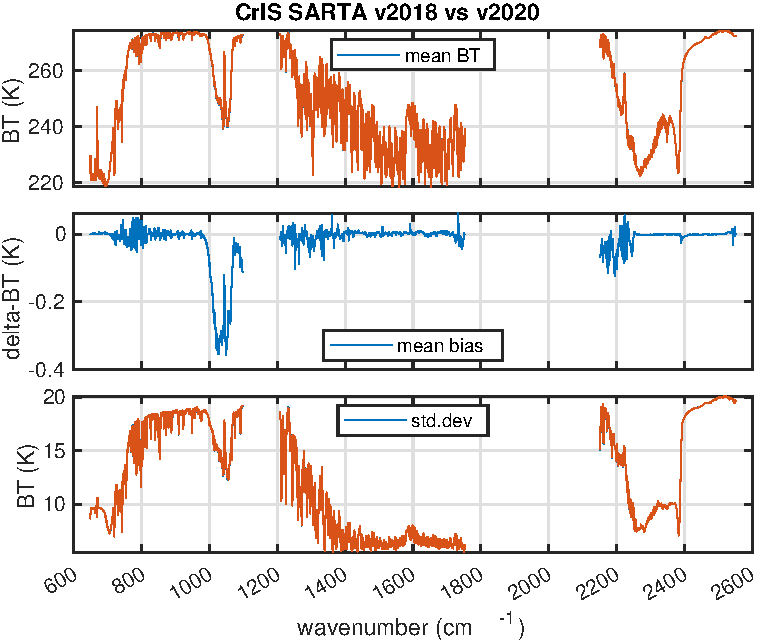
\includegraphics[width=0.75\linewidth]{./Figs/sarta_cris_hr_h2018_vs_h2020_r49_686_mn_stdaslp.pdf}
  \end{center}

\end{frame}
% ---------------------------------------------------------------------
\begin{frame}
  \frametitle{Updates 2: HDO}
  \begin{itemize}
    \item HDO lines have been modelled for all sensors in the MW and SW bands.
    \item Some validation has been successfully performed using ORACLES field data.
  \end{itemize}

% Side by side figures 
\begin{figure}
\begin{minipage}[c]{0.45\linewidth}
  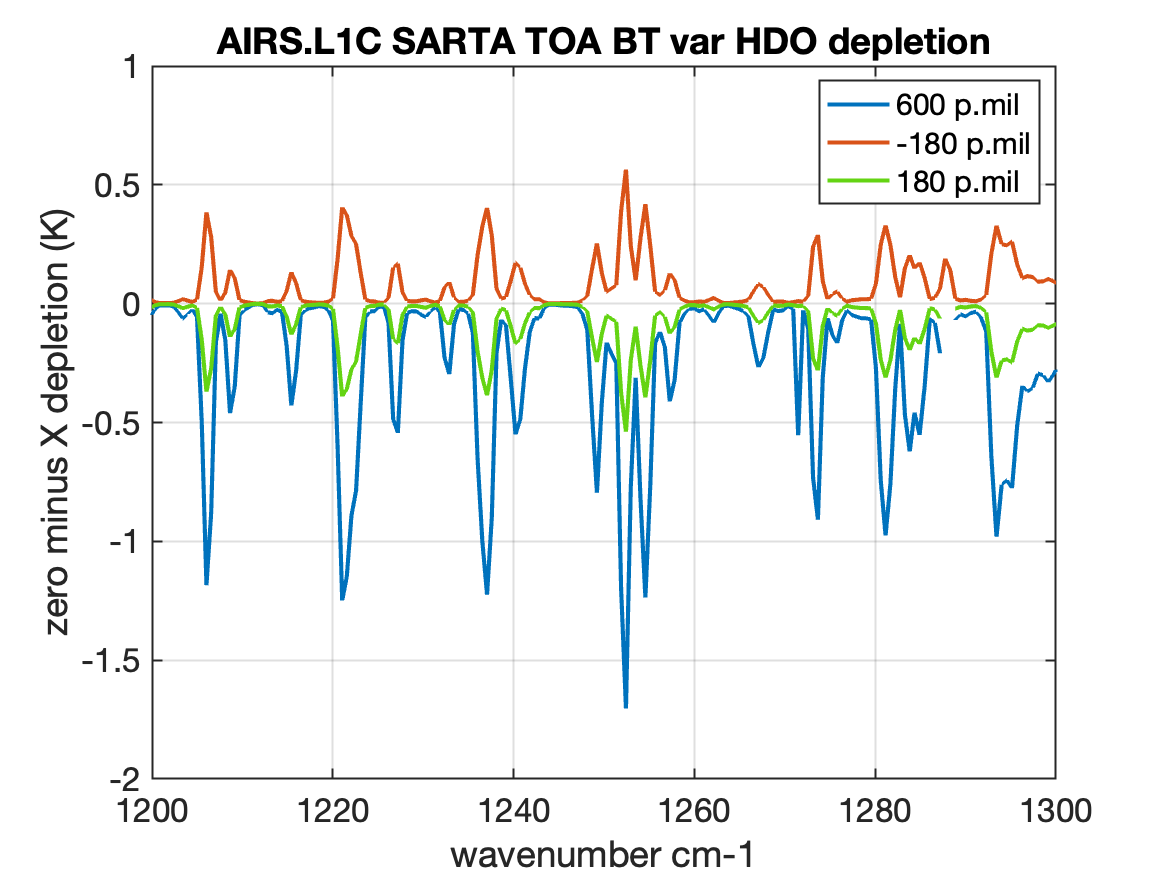
\includegraphics[width=\linewidth]{./Figs/airs_l1c_hdo_r49_mw_var_depletion.png}
  \caption{Simulated TOA BT changes due to varying HDO depletion, MW band.}
\end{minipage}
\hfill
\begin{minipage}[c]{0.45\linewidth}
  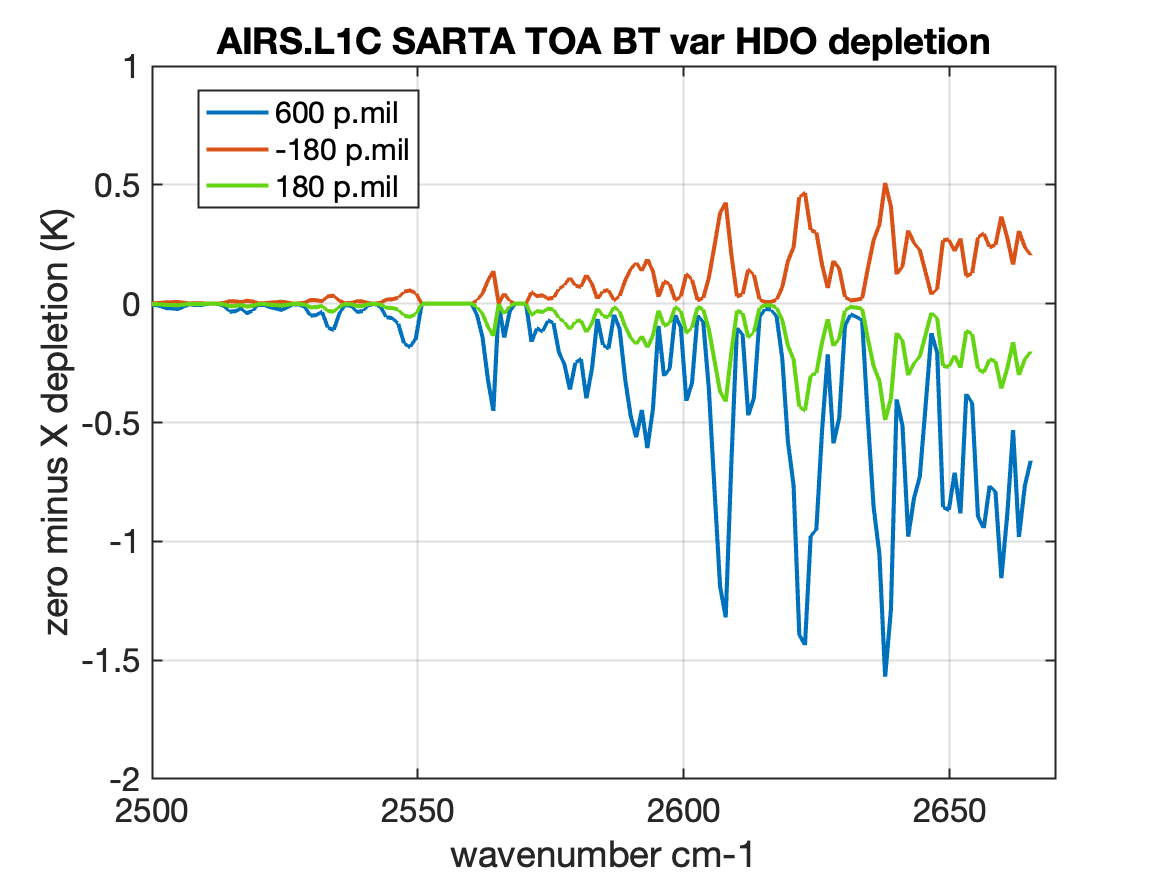
\includegraphics[width=\linewidth]{./Figs/airs_l1c_hdo_r49_sw_var_depletion.png}
  \caption{Simulated TOA BT changes due to varying HDO depletion, SW band}
\end{minipage}%
\end{figure}


\end{frame}

% ---------------------------------------------------------------------
\begin{frame}
  \frametitle{Updates 3: nonLTE}
  \begin{itemize}
  \item New vibrational temperatures in the 4.3 um CO2 band have been received from Peurtas et al
    Instituto Astrophysica de Andalucia (Sp.) that extend the range through sunset.
  \item The new (extended) nonLTE model includes 19 solar zenith angles instead of 6 previously
    increasing the atmospheric profile training set to 5586 from 1764.
  \end{itemize}

  \begin{center}
    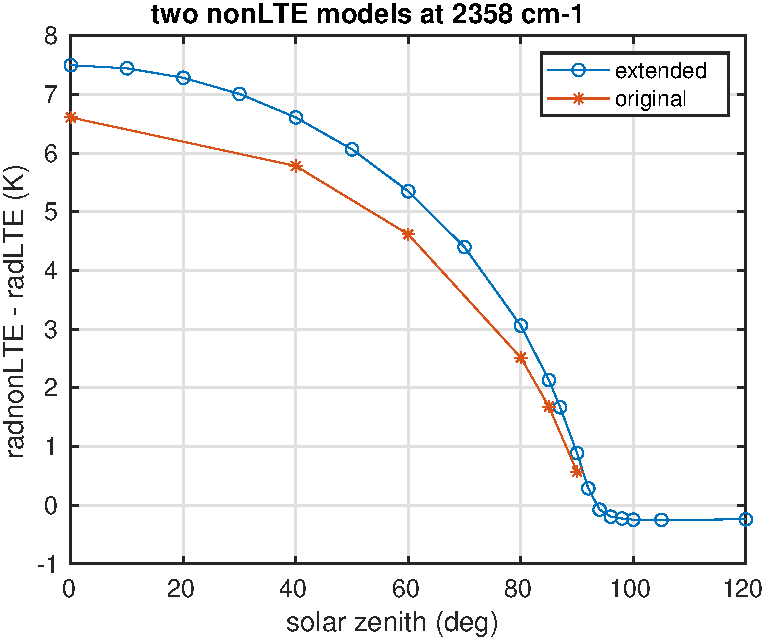
\includegraphics[width=0.5\linewidth]{./Figs/two_nlte_models_2358cm_vs_solzen.pdf}
  \end{center}
\end{frame}

% ---------------------------------------------------------------------
\begin{frame}
  \frametitle{Updates 3: nonLTE (2)}
  \begin{itemize}
  \item Fast coefficients using the original predictor set and several other predictors have been
    trialed.
  \item To-date there is little difference in the performance of the simulations.
\end{itemize}
  
% Side by side figures 
\begin{figure}
\begin{minipage}[c]{0.45\linewidth}
  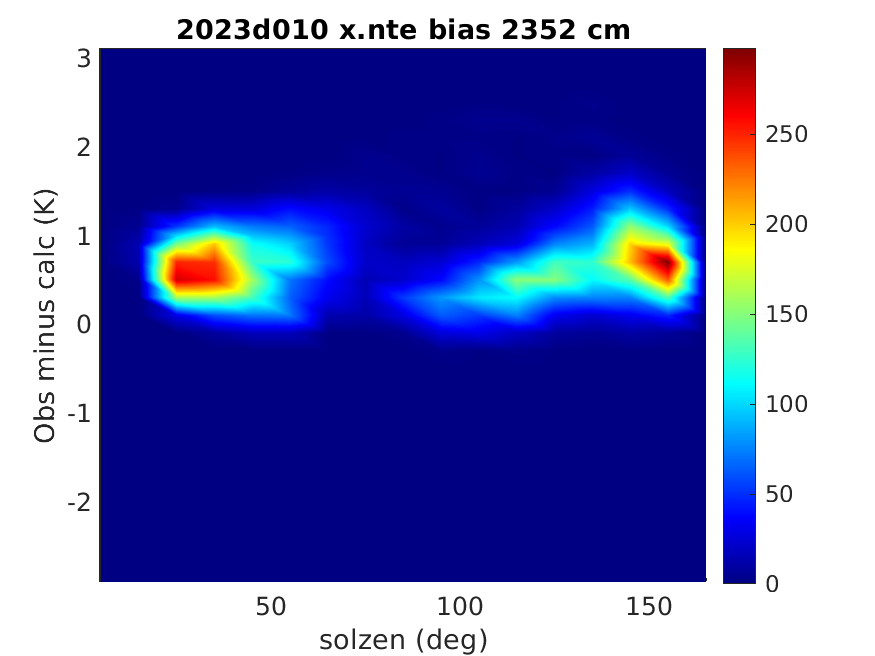
\includegraphics[width=\linewidth]{./Figs/2023d010_airs_xnte_bias_vs_solz_pcolor2.png}
  \caption{BT Bias vs solzen for a day of AIRS random obs at 2352 cm-1 (Untuned)}
\end{minipage}
\hfill
\begin{minipage}[c]{0.45\linewidth}
  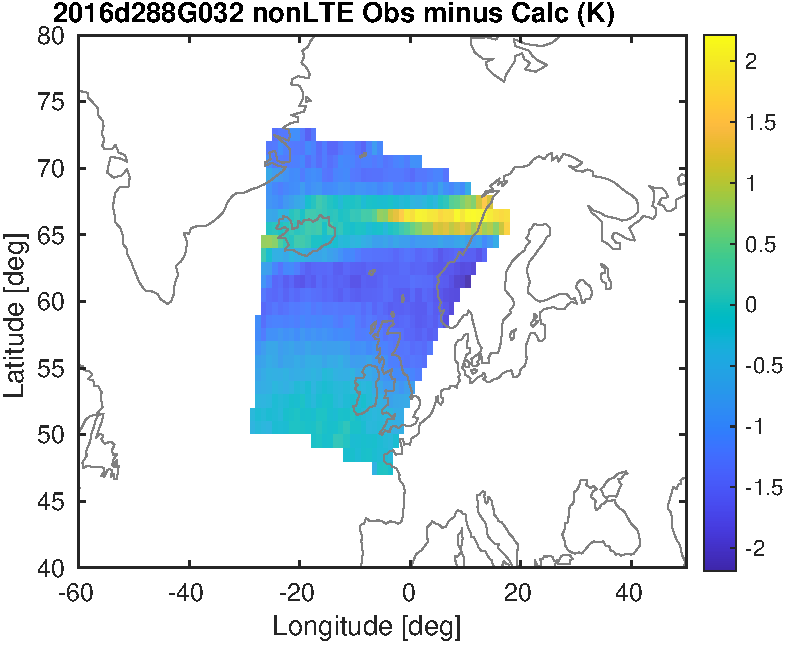
\includegraphics[width=\linewidth]{./Figs/2016d288g032_nlte_bias_obs_calc_map.pdf}
  \caption{Auroral Emission event, Bias BT at 2352 cm-1.}
\end{minipage}%
\end{figure}


\end{frame}      
% ---------------------------------------------------------------------
\begin{frame}
  \frametitle{Updates 4: Analytic Jacobians}
  \begin{itemize}
  \item Sergio has developed a method to compute Jacobians analytically using derivatives
    of the predictors, currently in experimetnal phase.
  \item Results compare well with kCARTA based Jacobians.
  \item SARTA analytic Jacs are ~60 x faster to compute than kCARTA Jacs. 
  \end{itemize}

  % Side by side figures 
\begin{figure}
\begin{minipage}[c]{0.45\linewidth}
  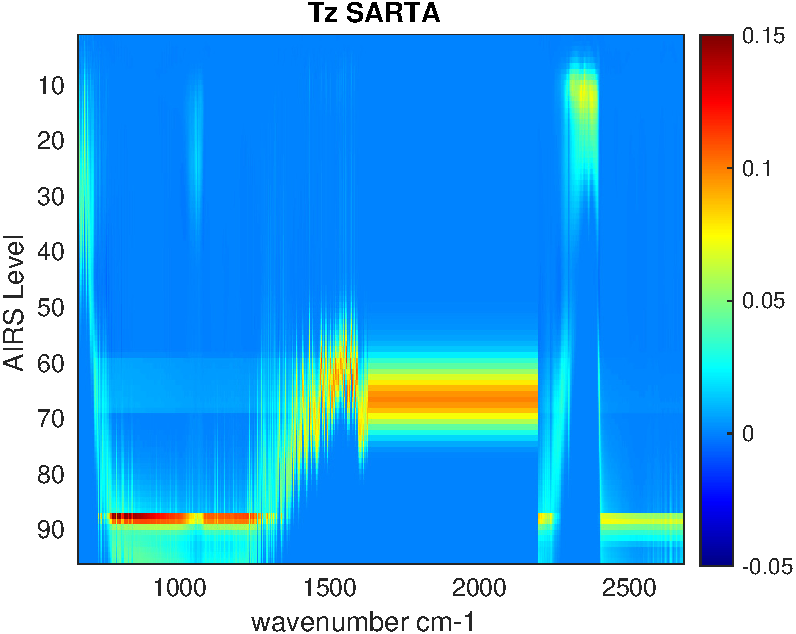
\includegraphics[width=\linewidth]{./Figs/jac_tz_sarta.pdf}
  \caption{T(z) Jacobian from SARTA analytic.}
\end{minipage}
\hfill
\begin{minipage}[c]{0.45\linewidth}
  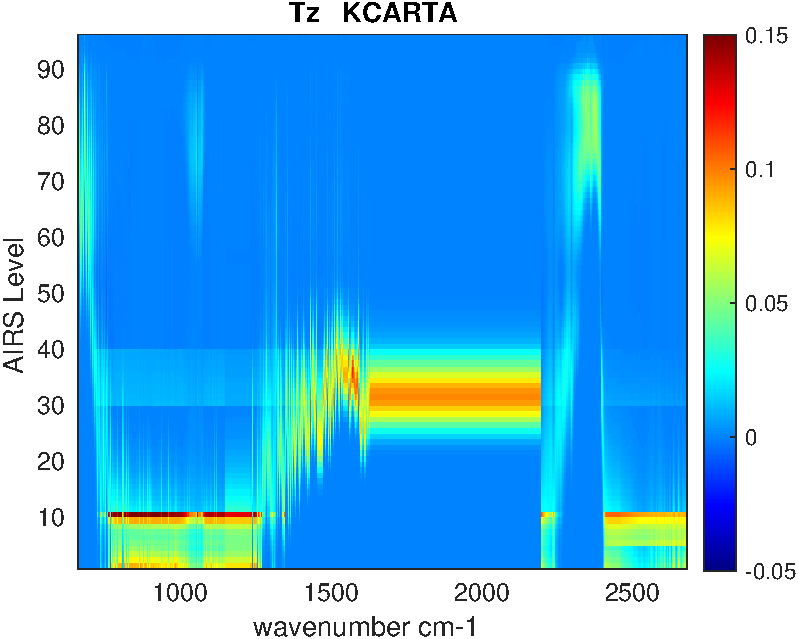
\includegraphics[width=\linewidth]{./Figs/jac_tz_kcarta.pdf}
  \caption{T(z) Jacobian from kCARTA.}
\end{minipage}%
\end{figure}

\end{frame}

% ---------------------------------------------------------------------
\begin{frame}
  \frametitle{Beneficial Future Changes}
  \begin{itemize}
    \item Make independent (agnostic) of file format types (HDF4, H5, netCDF).
    \item Simplify packaging and coefficient management.
    \item Extend/update training set, add machine learning if demonstrably beneficial.
    \item Adapt to the cloud and complete open-source migration (documentation).
    \item Re-package code with Julia or Python wrappers for wider community use.
    \item Include as part of CHIRP processing suite (cloud).

\end{itemize}
\end{frame}

% ---------------------------------------------------------------------
\begin{frame}
  \frametitle{Future 1: File format, Coefficient packaging}
  \begin{itemize}
    \item Currently there are 15 separate coefficient tables with many different predictors
      some predictors are common amongst some sets.
    \item Coefficients are stored as fortran binary files.
    \item Atmospheric state variables are supplied to SARTA as HDF-4 format files. 
  

  \end{itemize}
\end{frame}

% ---------------------------------------------------------------------
\begin{frame}
  \frametitle{Future 2: Adapt to the cloud}
  \begin{itemize}
    \item

  \end{itemize}
\end{frame}

% ---------------------------------------------------------------------
\begin{frame}
  \frametitle{Conclusions}
  \begin{itemize}
  \item SARTA remains a core component of research at UMBC/GESTAR-2 having been extended
    to simulation of radiances for several hyperspectral infrared sensors.
  \item SARTA radiometric accuracy continues to meet the needs for long term stabilty
    and climate studies.
  \item SARTA is particularly useful because of the speed of computation, together
    with parallization supports analysis of multi-decade, global sets of complete
    sensor spectra.
  \item Adapting SARTA to a complete opensource for use in the cloud should provide
    easy access to wide range of users. 

  \end{itemize}
\end{frame}

% ---------------------------------------------------------------------
\end{document}

